\documentclass[letter,11pt]{article}

\usepackage[spanish,es-nodecimaldot]{babel}
\usepackage[utf8]{inputenc}

\usepackage{lmodern}
\usepackage[T1]{fontenc}
\usepackage{textcomp}

\usepackage{framed}
\usepackage[svgnames]{xcolor}
\colorlet{shadecolor}{Gainsboro!50}

\usepackage{enumitem}
\usepackage{graphicx}
\usepackage{pstricks}

\usepackage{anysize}
\marginsize{3cm}{2cm}{2cm}{3cm}

\usepackage{siunitx}
\usepackage{amsmath}
\usepackage{array}
\usepackage{alltt}

\usepackage{fancyhdr}
\usepackage{lastpage}
\pagestyle{fancy}
\fancyhf{}
\fancyhead[LE,RO]{Física Básica II}
\fancyfoot[CO,CE]{\thepage\ de \pageref{LastPage}}

\special{papersize=215.9mm,279.4mm}

\usepackage[
    pdfauthor={Carlos Eduardo Caballero Burgoa},%
    pdftitle={Física Básica II},%
    pdfsubject={Tarea 8},%
    colorlinks,%
    citecolor=black,%
    filecolor=black,%
    linkcolor=black,%
    urlcolor=black,
    breaklinks]{hyperref}
\usepackage{breakurl}

\newcommand{\blankpage}{
\newpage
\thispagestyle{empty}
\mbox{}
\newpage
}

\renewcommand{\arraystretch}{1.2}

\begin{document}

\begin{center}
    {\Large \bf{Tarea \#8}}
\end{center}

Calcular el centro de masa de una lámina triangular de densidad superficial
uniforme.

\begin{figure}[!h]
\centering
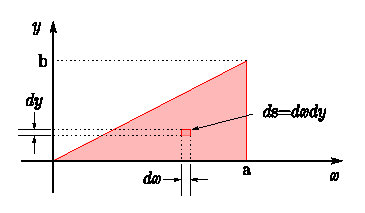
\includegraphics[scale=1.25]{resources/f1.eps}
\end{figure}

\textbf{Solución:} \\

Dada la ecuación del centro de masa:

\begin{equation}
    \vec{r}_{cm} = \frac{1}{M} \int_{M} \vec{r} \cdot dm
\label{base}
\end{equation}

Asumiendo la distribución homogénea de la masa sobre el material:
\begin{equation*}
    \sigma = \frac{dm}{ds} = ctte
\end{equation*}

Por tanto:
\begin{equation}
    dm = \sigma \cdot ds = \sigma \cdot dx \cdot dy
\label{dm}
\end{equation}

Reemplazando (\ref{dm}) en (\ref{base}):
\begin{equation*}
    \vec{r}_{cm} = \frac{1}{M} \int_{0}^{M} \vec{r} \cdot \sigma \cdot ds
\end{equation*}

Reemplazando $\vec{r}$ por sus componentes:
\begin{equation*}
    \vec{r}_{cm} = \frac{1}{M} \int_{0}^{S} (x \hat{i} + y \hat{j}) \cdot \sigma \cdot ds = \frac{\sigma}{M} \int_{0}^{a} \int_{0}^{y} (x \hat{i} + y \hat{j}) \cdot dx \cdot dy
\end{equation*}

Sabiendo que la relación entre $x$ y $y$ es:
\begin{equation*}
    y = \frac{b}{a} x
\end{equation*}

Para $\hat{i}$ obtenemos:
\begin{equation*}
    x_{cm} = \frac{\sigma}{M} \int_{0}^{a} \int_{0}^{\frac{b}{a}x} x \cdot dy \cdot dx = \frac{\sigma}{M} \int_{0}^{a} x \left(\int_{0}^{\frac{b}{a}x} dy \right) dx = \frac{\sigma}{M} \int_{0}^{a} x \cdot y\Biggr|_{0}^{\frac{b}{a}x} dx
\end{equation*}
\begin{equation*}
    x_{cm} = \frac{\sigma}{M} \int_{0}^{a} x \left(\frac{b}{a} x\right) dx = \frac{\sigma}{M} \int_{0}^{a} \frac{b}{a} x^2 dx = \frac{\sigma}{M} \frac{b}{a} \int_{0}^{a} x^2 dx
\end{equation*}
\begin{equation*}
    x_{cm} = \frac{\sigma}{M} \frac{b}{a} \frac{x^3}{3}\Biggr|_{0}^{a} = \frac{\sigma}{M} \left(\frac{b}{a} \frac{a^3}{3}\right) = \frac{\sigma}{M} \left(\frac{a^2 b}{3}\right)
\end{equation*}

Para $\hat{j}$ obtenemos:
\begin{equation*}
    y_{cm} = \frac{\sigma}{M} \int_{0}^{a} \int_{0}^{\frac{b}{a}x} y \cdot dy \cdot dx = \frac{\sigma}{M} \int_{0}^{a} \left(\int_{0}^{\frac{b}{a}x} y \cdot dy \right) dx = \frac{\sigma}{M} \int_{0}^{a} \frac{y^2}{2} \Biggr|_{0}^{\frac{b}{a}x} dx
\end{equation*}
\begin{equation*}
    y_{cm} = \frac{\sigma}{M} \int_{0}^{a} \frac{1}{2} \frac{b^2}{a^2} x^2 dx = \frac{\sigma}{M} \frac{1}{2} \frac{b^2}{a^2} \int_{0}^{a} x^2 dx
\end{equation*}
\begin{equation*}
    y_{cm} = \frac{\sigma}{M} \frac{1}{2} \frac{b^2}{a^2} \frac{x^3}{3} \Biggr|_{0}^{a} = \frac{\sigma}{M} \left( \frac{1}{2} \frac{b^2}{a^2} \frac{a^3}{3} \right) = \frac{\sigma}{M} \left( \frac{ab^2}{6} \right)
\end{equation*}

\vspace{0.5cm}
Uniendo ambas componentes, obtenemos:
\begin{equation}
    \vec{r}_{cm} = \frac{\sigma}{M} \left( \frac{a^2 b}{3} \right) \hat{i} + \frac{\sigma}{M} \left( \frac{a b^2}{6} \right) \hat{j}
\label{vector}
\end{equation}

A partir de la ecuación (\ref{dm}) sabemos que:
\begin{equation*}
    M = \sigma \cdot s = \sigma \frac{a \cdot b}{2}
\end{equation*}

Despejando $M$ de la ecuación (\ref{vector}), obtenemos:
\begin{equation*}
    \vec{r}_{cm} = \frac{2 a}{3} \hat{i} + \frac{b}{3} \hat{j}
\end{equation*}

\end{document}

